%%
%% Beuth Hochschule für Technik --  Abschlussarbeit
%%
%% Anhang
%%
%%%%%%%%%%%%%%%%%%%%%%%%%%%%%%%%%%%%%%%%%%%%%%%%%%%%%%%%%%%%%%%%%%%%%

\chapter{Zusätze}

\setglossarysection{section}
\printglossary[type=\acronymtype,title=Abkürzungen]


\section{Quelltext}
\label{section:quelltext}

\lstinputlisting[language=XML, label=lst:aurorborealisdeoployconf, caption=Aurora Borealis Konfiguration für die Verteilung]{anhangQuelltext/borealismytestdist-deploy.xml}

\lstinputlisting[language=XML, label=lst:aurorborealisqueryconf, caption=Aurora Borealis Konfiguration für die Abfragen]{anhangQuelltext/borealismytestdist.xml}

\lstinputlisting[language=C++, label=lst:aurorborealismytest, caption=Aurora Borealis Testanwendung]{anhangQuelltext/mytestdist.cc}

\lstinputlisting[language=JAVA, label=lst:WordCountTopology, caption=Apache Storm WordCount Demo]{anhangQuelltext/WordCountTopology.java}

\lstinputlisting[language=JAVA, label=lst:kafkaProducer, caption=Apache Kafka Producer Beispiel]{anhangQuelltext/kafkaProducer.java}

\lstinputlisting[language=JAVA, label=lst:kafkaConsumer, caption=Apache Kafka Consumer Beispiel]{anhangQuelltext/kafkaConsumer.java}

\lstinputlisting[language=JAVA, label=lst:s4HelloAppProcessingElement, caption=Apache S4 Processing Element Beispiel]{anhangQuelltext/s4HelloAppProcessingElement.java}

\lstinputlisting[language=JAVA, label=lst:s4HelloAppProcessingElementInstance, caption=Apache S4 Processing Element Instanz Beispiel]{anhangQuelltext/s4HelloAppProcessingElementInstance.java}

\lstinputlisting[language=JAVA, label=lst:s4HelloInputAdapter, caption=Apache S4 HelloInputAdapter Beispiel]{anhangQuelltext/s4HelloInputAdapter.java}

\section{Zusatz Systemarchitektur}
\label{section:zusSystemarchitektur}

\begin{figure}[htb!]
\centering
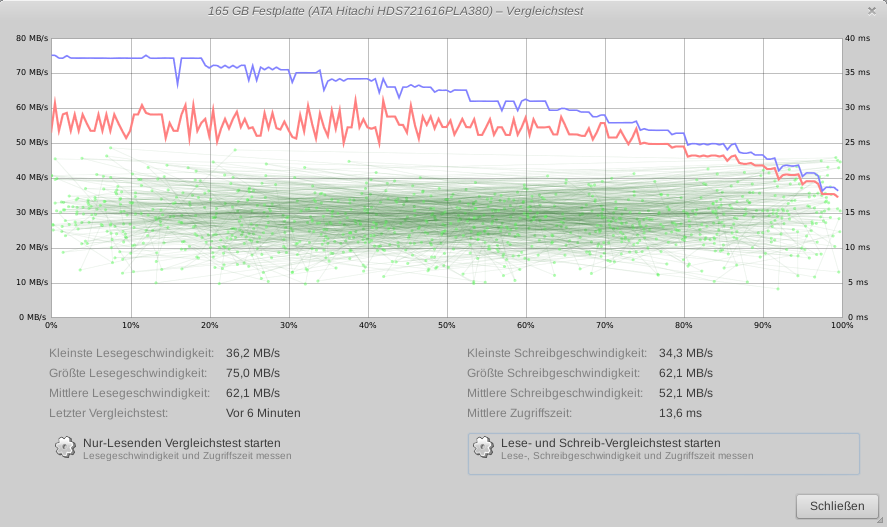
\includegraphics[width=1.0\textwidth]{bilder/LaufwerkstestHitachi165GB.png}
\caption{Leistungstest Festplatte Hitachi
\label{fig:festplatteLeistungstest}}
\end{figure}



\section{Zusatz Prototyp Dokumentation}
\label{section:zusPrototypDokumentation}

\lstinputlisting[label=lst:stormBroker, caption=Broker für Apache Storm]{anhangQuelltext/server.js}
\lstinputlisting[label=lst:graphJs, caption=D3 Graph]{anhangQuelltext/graph.js}
\lstinputlisting[label=lst:mainJs, caption=Auszug Main Javascript]{anhangQuelltext/main.js}
\lstinputlisting[label=lst:WebSocketClientFactory, caption=Java Factory WebSocketClient]{anhangQuelltext/WebSocketClientFactory.java}

\section{Installationsanleitung Aurora/Borealis}
\label{sec:aurborinstall}


In dieser Anleitung wird die Installation von Aurora Borealis in kleinen Unterkapiteln vorgestellt. Diese Anleitung setzt ein Vorwissen in der Verwendung und Administration von Linux voraus. Zudem wird Erfahrung von Erzeugen von Anwendungen aus Quelltext benötigt. Zum Beispiel können Konflikte auftreten, wenn neue Versionen von Bibliotheken benötigt werden. Dabei müssen die Abhängigkeiten beachtet und abhängige Konflikte aufgelöst werden. Bevor das Erstellen der Anwendung beginnt werden zuerst die Voraussetzungen bestimmt und erläutert. Anschließend wird mit Quelltextfragementen und Kommandozeilenausschnitten schrittweise die Eingabe und Ausgabe gezeigt.


\subsection{Voraussetzungen am Betriebssystem}

Die Installation von Aurora Borealis benötigt ein auf linuxbasiertes Betriebsystem. Auf dem Betriebssystem Microsoft Windows wurde eine Erstellung des Quelltextes von Aurora Borealis bisher nicht durchgeführt. Zum Zeitpunkt der Erstellung dieser Anleitung wird versucht ein Ist-Zustand der Anwendung aufzunehmen. Für das Verteilte System Aurora Borealis wird die Linuxdistribution Debian benutzt.


\subsection{Voraussetzung Erstellsystem}

Einige Pakete bzw. Bibliotheken werden für das Erstellen von Aurora Borealis benötigt. Als Paketverwaltung wird unter Debian \textit{apt} benutzt. Mit dem Befehl \textit{apt-get} können Pakete dem Betriebssystem aus dem Standard Debian Paket-Repository hinzugefügt werden. Folgende Liste zeigt benötigte Pakete für das Erstellen von Aurora Borealis:

\begin{itemize}
	\item build-essentials (gcc, g++, configure, make)
	\item ccache
	\item antlr
	\item libxerces-c3.1 (Xerces-c: Used by Borealis to parse XML)
	\item libtool
	\item autoconf
	\item automake
	\item libdb5.1 (Berkeley-Db)
	\item glpk (GNU Linear Programming Kit)
	\item gsl (GNU Scientific Library - collection of routines for numerical analysis: used for predictive queries)
	\item opencv (open source computer vision: used for array processing)
	\item doxygen (serves to generate documentation)
	\item openjdk-7-jdk (java 7)
\end{itemize}

Da die letzte Version von Aurora Borealis aus dem Jahr 2008 ist, gibt es beim Erstellen mit neueren Versionen von \textit{gcc} und \textit{g++} Fehler. 
Damit die neue Version von \textit{gcc} benutzt werden kann muss der Quelltext der Version aus 2008 angepasst werden. Eine erste Anpassung wurde versucht durchzuführen. Zum Beispiel sind bestimmte Standardmethoden direkt angegeben worden. Trotzdem wurden weiterführende Fehler gefunden. Als Fehler wird \textit{missing \#include} gemeldet. Im \textit{borealis} Verzeichnis sind 239 \textit{Makefiles} vorhanden. Alle \textit{Makefiles} und die darin verbundenen Quelltext-Dateien müssen auf die neue Version geprüft werden. Eine Stabile Version mit den neuen Anpassungen kann nur durch effektive Testläufe gewährleistet werden. Um den Quelltext von Aurora Borealis nicht anzupassen kommt die ältere Version 4.0 von Debian zum Einsatz. In diesem Fall muss die Liste von benötigten Paketen angepasst werden:

\begin{itemize}
	\item build-essentials (gcc, g++, configure, make)
	\item ccache
	\item antlr
	\item libxerces27 (Xerces-c: Used by Borealis to parse XML)
	\item libtool
	\item autoconf
	\item automake
	\item libdb (Berkeley-Db)
	\item glpk (GNU Linear Programming Kit)
	\item gsl (GNU Scientific Library - collection of routines for numerical analysis: used for predictive queries)
	\item opencv (open source computer vision: used for array processing)
	\item doxygen (serves to generate documentation)
	\item sun-java5-jdk (Java 1.5 von SUN)
	\item libexpat1-dev
	\item ibreadline5-dev
\end{itemize}


\subsection{Quelltext von Aurora Borealis herunterladen}

Die Datei liegt nicht in einer öffentlichen Versionsverwaltung, sondern kann als Archive von der Brown University unter folgendem Link heruntergeladen werden:
\url{http://www.cs.brown.edu/research/borealis/public/download/borealis_summer_2008.tar.gz} \\
Alternativ liegt der Quelltext und das Installationsmedium Debian 4.0 als \gls{glo:iso} 9660 Abbild im Ordner \textit{anhangSoftwareZusatz}. Nachdem die Anwendung im Verzeichnis \textit{/opt} liegt kann sie im gleichen Verzeichnis entpackt werden. Im Verzeichnis liegen anschließend zwei Unterordner \textit{borealis} und \textit{nmstl}.


\subsection{Kommandozeile Umgebungsvariablen festlegen}

Unter Debian wird für die Kommandozeile die Shell \textit{Bash} eingesetzt. Wenn eine Shell eröffnet wird, wird die Datei \textit{.bashrc} im Benutzerverzeichnis aufgerufen. Darin werden Benutzerabhängige Konfigurationen abgelegt. Die Umgebungsvariablen für Aurora Borealis werden im folgenden Abschnitt gezeigt:
\begin{verbatim}
alias debug='export LOG_LEVEL=2'
alias debug0='export LOG_LEVEL=0'
export PATH=${PATH}:/opt/nmstl/bin:/${HOME}/bin
export CLASSPATH='.:/usr/share/java/antlr.jar:$CLASSPATH'
export JAVA_HOME=$(readlink -f /usr/bin/javac | sed "s:/bin/javac::")
export PATH=${JAVA_HOME}/bin:${PATH}
export CXX='ccache g++'
export CVS_SANDBOX='/opt'
export INSTALL_BDB='/usr'
export INSTALL_GLPK='/usr'
export INSTALL_GSL='/usr'
export INSTALL_ANTLR='/usr'
export INSTALL_XERCESC='/usr'
export INSTALL_NMSTL='/usr/local'
export LD_LIBRARY_PATH='/usr/lib'
export ANTLR_JAR_FILE='/usr/share/java/antlr.jar'

mkdir -p bin
alias bbb='/opt/borealis/utility/unix/build.borealis.sh'
alias bbbt='/opt/borealis/utility/unix/build.borealis.sh -tool.head
 -tool.marshal'
alias retool='/bin/cp -f ${CVS_SANDBOX}/borealis/tool/head/BigGiantHead
 ${HOME}/bin; /bin/cp -f ${CVS_SANDBOX}/borealis/tool/marshal/marshal
 ${HOME}/bin'
\end{verbatim}


\subsection{Notwendige Quelltext Anpassung}

Beim Erzeugen wird unter anderen Paketen auch \gls{glo:antlr} benutzt. Während der Erstellens findet ein Fehler auf. Bei der Konfiguration für das \textit{Makefile} wurde ein Pfad fest einprogrammiert. Dieser feste Pfad wird nun durch einen Variable in die Umgebungsvariable \textit{ANTLR\_JAR\_FILE} ausgelagert. Dazu muss in der Datei \textit{/opt/borealis/src/configure.ac} der Inhalt an der Stelle ANTLR\_JAR\_FILE= mit \textit{\$ANTLR\_JAR\_FILE} nach dem Gleichzeichen ausgetauscht werden.


\subsection{Erzeugen von NMSTL}

Borealis benutzt eine angepasste Version von \gls{glo:nmstl}. Im Verzeichnis \textit{/opt/nmstl} werden nun folgende Befehle nacheinander ausgeführt:

\begin{verbatim}
autoconf
./configure
make
make install
\end{verbatim}


\subsection{Erzeugen von Borealis}

In das Verzeichnis \textit{/opt/borealis} zurückspringen und folgende Befehle nacheinander ausführen:

\begin{verbatim}
bbb
bbbt
retool
make install
\end{verbatim}


\subsection{Zusätzliche Informationen}
Der Support für Aurora Borealis ist seit 2008 eingestellt. Weitere Informationen stehen unter folgendem Link:
\url{http://cs.brown.edu/research/borealis/public/install/install.borealis.html}

\section{Installationsanleitung Apache Storm}
\label{sec:storminstall}


In diesem Kapitel wird die Installation von Apache Storm in kleinen Unterkapiteln vorgestellt. Die Anleitung setzt ein Wissen in der Verwendung, Administration und Erzeugen von Anwendungen unter dem Betriebssystem Linux voraus. Zuerst werden Voraussetzungen bestimmt und erläutert. Anschließend wird der Start eines Clusters gezeigt. Zuletzt wird eine Beispiel-Anwendung \textit{WordCount} im \textit{local cluster mode} ausgeführt.


\subsection{Voraussetzungen am Betriebssystem}

Als Betriebssystem wird in dieser Anleitung Linux mit der Deistribution Ubuntu 13.10 verwendet. Apple Mac OS X und Microsoft Windows mit einer Cygwin-Umgebung werden in dieser Anleitung nicht betrachtet. Unter Ubuntu wird für die Installation von Paketen das Kommandozeilen-Werkzeug \textit{aptitude }eingesetzt.


\subsection{Paketabhängigkeiten}

Einige Pakete benötigt Apache Storm zur Laufzeit bzw. werden zum Erzeugen gebraucht. Die folgende Liste stellt die notwendigen Pakete dar:

\begin{itemize}
	\item zookeeper
	\item libtool
	\item autoconf
	\item automake
	\item openjdk-7-jdk
	\item zeromq (evt. nicht im Linux Repository)
	\item jzmq (evt. nicht im Linux Repository)
\end{itemize}

Falls die Pakete zu ZeroMQ in den Paketquellen fehlen, müssen beide manuell erzeugt und dem Betriebssystem hinzugefügt werden. Folgende Kommandozeilen zeigen das Herunterladen, Erzeugen und Bereitstellen von ZeroMQ schrittweise:
\begin{verbatim}
wget download.zeromq.org/zeromq-3.2.4.tar.gz
tar xvfz zeromq-3.2.4.tar.gz
./configure
make 
make install
ldconfig
\end{verbatim}

Apache Storm benutzt zur Kommunikation mit ZeroMQ Java-Bindings. Folgende Kommandozeilenaufrufe müssen zur Installation schrittweise ausgeführt werden:
\begin{verbatim}
wget github.com/zeromq/jzmq/archive/master.zip
./autogen.sh
./configure
make
\end{verbatim}


\subsection{Storm Konfiguration}

Apache Storm in das Verzeichnis /opt herunterladen, entpacken und einen Link \textit{storm} erstellen.
\begin{verbatim}
wget http://apache.openmirror.de/incubator/storm/
	apache-storm-0.9.1-incubating/apache-storm-0.9.1-incubating-src.zip
unzip apache-storm-0.9.1-incubating-src.zip
ln -s storm apache-storm-0.9.1-incubating-src.zip
\end{verbatim}

Die Konfigurationsdatei /opt/storm/conf/storm.yaml öffnen und folgenden Eintrag hinzufügen:
\begin{verbatim}
storm.local.dir: "/opt/storm"
\end{verbatim}


\subsection{Cluster starten}

Zookeeper muss bereits im Hintergraund als Dienst laufen, damit das Storm Cluster starten kann.

Mit folgendem Befehl kann der Zookeeper Dienst auf Aktivität gerpüft werden.
\begin{verbatim}
./zkCli.sh -server 127.0.0.1:2181 
\end{verbatim}

Die folgenden Schritte zeigen nacheinander den Start der Storm Komponenten:

\begin{verbatim}
/opt/storm/bin/storm nimbus
/opt/storm/bin/storm supervisor
/opt/storm/bin/storm ui
\end{verbatim}


\subsection{WordCount Demo im local cluster mode}

Mit git wird zuerst die Beispiel Anwendung WordCount in ein lokales Verzeichnis dublizieren:

\begin{verbatim}
git clone git://github.com/apache/incubator-storm.git
\end{verbatim}

Die Anwendung WordCountTopology wird mit Apache Maven im storm cluster bereitgestellt und ausgeführt:

\begin{verbatim}
mvn -f m2-pom.xml compile exec:java -Dexec.classpathScope=compile 
-Dexec.mainClass=storm.starter.WordCountTopology
\end{verbatim}

Da keine Argumente bei der Ausführung übergeben werden, wird als \textit{cluster} der \textit{LocalCluster} benutzt. In der Java Klasse \textit{WordCountTopology} wird in der \textit{main}-Methode entschieden, ob der LocalCluster benutzt wird. Als Ausgabe werden während der Verarbeitung Log Informationen ausgegeben. Eine Erfolgmeldungs wird ausgegeben, falls das Erstellen und Ausführen auf dem Cluster erfolgreich durchgeführt wurde.

\section{Installationsanleitung Apache Kafka}
\label{section:kafkainstall}


Dieses Kapitel beschreibt schrittweise die Installation von Apache Kafka. Die Installation erfordert Kenntnisse in der Installation und Administration von Anwendungen unter dem Betriebssystem Linux. Eine Installation unter dem Betriebssystem Unix, Max OS X und Microsoft Windows wird in dieser Arbeit nicht behandelt. Bevor die Installation beginnen kann, werden zuerst Voraussetzung an das Betriebssystem aufgezählt. Im Kapitel Installation wird der Quelltext kompiliert und ein erster Start von Kafka wird gezeigt. Abschließend wird eine Konfiguration für ein Kafka Single Broker Cluster vorgestellt und Beispiel zwischen einem Producer, dem Nachrichtenerzeuger und einem Consumer, dem Nachrichtenempfänger gezeigt.


\subsection{Voraussetzungen in Linux}

Als Linux Distribution wird Debian 7 verwendet. Da Apache Kafka auf Scala basiert, werden folgende Linux-Pakete benötigt:

\begin{itemize}
	\item zookeeper
	\item scala
	\item openjdk-7-jdk	
\end{itemize}

Das Hinzufügen der Linux-Pakete kann mit der Paketverwaltung \textit{apt-get} oder mit \textit{aptitude} erfolgen. Weitere Paket-Abhängigkeiten werden automatisch vorgeschlagen. Die Installation der Paket-Abhängigkeiten ist zwingend und Konflikte müssen aufgelöst werden.  

Um die notwendige Abhängigkeiten, wie unter Java mit Maven\footnote{Maven: Java Build Werkzeug \url{http://maven.apache.org/}} unter Scala aufzulösen, wird das Werkzeug \gls{glo:sbt} von der Webseite \url{http://www.scala-sbt.org/download.html} benötigt. Zunächst wird in das Verzeichnis \textit{opt} gewechselt und das Archiv \textit{sbt} heruntergeladen. Anschließend wird das Archiv entpackt und Drei \textit{sbt}-Dateien werden im System global bereitgestellt:

\begin{verbatim}
cd /opt
wget http://dl.bintray.com/sbt/native-packages/sbt/0.13.5/sbt-0.13.5.tgz
tar xvfz sbt-0.13.5.tgz
cd sbt
mv sbt /usr/local/bin
mv sbt-launch-lib.bash /usr/local/bin
mv sbt-launch.jar /usr/local/bin
\end{verbatim}

Mit \textit{sbt console} kann eine Scala-Shell eröffnet werden. Das \textit{Build}-Werkzeug ist korrekt bereitgestellt, wenn nach dem Aufruf eine Scala-Eingabezeile erscheint. Mit dem Befehl \textit{:quit} kann die Scala-Eingabeumgebung wieder geschlossen werden. Als nächstes wird der Quelltext von Apache Kafka heruntergeladen, entpackt, Apache Kafka kompiliert und der Packet-Cache aktualisiert. Beim ersten Aufruf von \textit{sbt} werden benötigte Scala-Bibliotheken automatisch heruntergeladen.

\begin{verbatim}
cd /root
wget http://apache.openmirror.de/kafka/0.8.1.1/kafka-0.8.1.1-src.tgz 
cd kafka-0.8.1.1
gradlew jar
sbt update
sbt package
sbt sbt-dependency
\end{verbatim}

Falls Zookeeper unter Debian in der Standardkonfiguration noch nicht ausgeführt wird, kann mit "`\textit{/etc/init.d/zookeeper start}"' der Dienst gestartet werden.

\subsection{Start Single Broker Cluster}

Im Kafka-Verzeichnis \textit{config} liegen die Konfigurationen für den Betrieb eines Clusters. In der Datei \textit{server.properties} wird eine eindeutige Nummer für den \textit{Broker}, eine Log-Datei und eine Referenz zum \textit{Zookeeper-Server} angegeben.

\begin{verbatim}
Broker.id=0
log.dir=/tmp/kafka.log
zookeeper.connect=localhost:2181
\end{verbatim}

Folgender Befehl startet den Kafka-Server in den Standardeinstellungen:
\begin{verbatim}
bin/kafka-server-start.sh config/server.properties
\end{verbatim}


\subsection{Producer und Consumer ausführen}

Sobald der Single Broker Cluster läuft kann mit den Shell-Skripten in separaten Shells ein Konsolen-Producer und ein Konsolen-Consumer gestartet werden.

Starten einer Topics:
\begin{verbatim}
bin/kafka-Console-topic.sh --replica 2 --zookeeper localhost:2181
 --topic contop
\end{verbatim}

Starten einer Producers. Nach dem Start kann sofort in der Eingabezeile etwas eingetippt werden.
\begin{verbatim}
bin/kafka-Console-producer.sh --broker-list localhost:9092 --sync 
 --topic contop
\end{verbatim}

Starten einer Consumers. Sobald der Consumer gestartet wurde, werden die Eingaben vom Producer auf der Kommandozeile ausgegeben.
\begin{verbatim}
bin/kafka-Console-consumer.sh --zookeeper localhost:2181 --from-beginning
 --topic contop 
\end{verbatim}
\section{Installationsanleitung Apache Flume}
\label{section:flumeinstall}


In diesem Kapitel wird die Installation von Apache Flume schrittweise gezeigt. Für die Installation von Apache Flume wird die aktuelle Version 1.5.0.1 verwendet. Als Betriebssystem wird Linux mit der Distribution Debian 7 eingesetzt. Eine Kompilation der Anwendung Apache Flume wird nicht durchgeführtm, daher werden einfache Kenntnisse in der Administration und Pflege von Linux-Betriebssystemen in der Shell Bash vorausgesetzt. Nach der Installation wird eine kleine Anwendung eines Apache Flume Agenten vorgestellt. 

Für den Einsatz von Apache Flume ist eine Java-Umgebung-Laufzeitumngebung notwendig. Die Installation der Debian Java7-Pakets kann mit Werkzeug \textit{aptitude} oder \textit{apt-get} durchgeführt werden.

\begin{verbatim}
aptitude install openjdk-7-jdk	
\end{verbatim}

Anschließend wird die vorkompilierte Apache Flume Anwenundung als Archiv vom Apache Server in das Verzeichnis \textit{/opt} heruntergeladen und entpackt. Abschließend wird das entpackte Verzeichnis in den Namen \textit{flume} umbenannt:

\begin{verbatim}
cd /opt
wget http://www.apache.org/dist/flume/1.5.0.1/apache-flume-1.5.0.1-bin.tar.gz
tar xvfz apache-flume-1.5.0.1-bin.tar.gz
mv apache-flume-1.5.0.1-bin.tar.gz flume
\end{verbatim}

\subsection{Apache Flume Konfiguration}
\label{section:flumeKonfiguration}

Damit Apache Flume ordentlich ausgeführt wird, muss die Konfiguration von Apache Flume für die Java-Umgebung und die JAVA\_HOME-Variable gesetzt sein.
Im Unterverzeichnis conf befinden sich template-Konfigurationsdateien. Zuerst werden die Template-Dateien in Konfigurationsdateien kopiert und anschließend bearbeitet:

\begin{verbatim}
cp flume-env.sh.template flume-env.sh
cp flume-conf.properties.template flume-conf.properties
\end{verbatim}

Mit einem Texteditor wie zum Beispiel vim, emacs oder nano können Dateien bearbeitet werden:
\begin{verbatim}
vim flume-env.sh
\end{verbatim}

Die folgende Konfigurationsdatei \textit{flume-env.sh} stellt ein Beispiel für Apache Flume dar. Zum einen wird die JAVA\_HOME-Variable mit dem richtigen Pfad zum Java-Installationsort gesetzt und zum Anderen wird das Moninoring über JMX mit Optionen für den Java Heap bereitgestellt.

\begin{lstlisting}[language=BASH, label=lst:flumeEnv, caption=Apache Flume Konfiguration]
# Licensed to the Apache Software Foundation (ASF) under one
# or more contributor license agreements.  See the NOTICE file
# distributed with this work for additional information
# regarding copyright ownership.  The ASF licenses this file
# to you under the Apache License, Version 2.0 (the
# "License"); you may not use this file except in compliance
# with the License.  You may obtain a copy of the License at
#
#     http://www.apache.org/licenses/LICENSE-2.0
#
# Unless required by applicable law or agreed to in writing, software
# distributed under the License is distributed on an "AS IS" BASIS,
# WITHOUT WARRANTIES OR CONDITIONS OF ANY KIND, either express or implied.
# See the License for the specific language governing permissions and
# limitations under the License.

# If this file is placed at FLUME_CONF_DIR/flume-env.sh, it will be sourced
# during Flume startup.

# Enviroment variables can be set here.

JAVA_HOME=/usr/lib/jvm/java-1.7.0-openjdk-amd64

# Give Flume more memory and pre-allocate, enable remote monitoring via JMX
JAVA_OPTS="-Xms100m -Xmx200m -Dcom.sun.management.jmxremote"

# Note that the Flume conf directory is always included in the classpath.
#FLUME_CLASSPATH=""
\end{lstlisting}

Die Konfigurationsdatei \textit{flume-conf.properties} kann verändert werden, wenn das Standardprotokollverhalten unerwünscht ist. In der Standardeinstellung wird über einen eigenen Agenten mit Log4j im Verzeichnis \textit{logs} und der Datei \textit{flume.log} protokolliert. Weitere Einstellungen können in der Datei \textit{log4j.properties} vorgenommen werden.

Folgender Aufruf zeigt Optionen für einen Apache Flume-Aufruf aus dem \textit{flume}-Verzeichnis:
\begin{verbatim}
 bin/flume-ng --help
\end{verbatim}

\subsection{Apache Flume Single-Node Beispiel}
\label{section:flumeBeispiel}

Folgendes Beispiel wird an dieser Stelle von der Apache Flume 1.5.0 User Guide \citeint{flume:userGuide} wieder gegeben und wird im Verzeichnis \textit{conf} als \textit{example.conf} abgepeichert.

\begin{lstlisting}[language=BASH, label=lst:flumeExample, caption=Apache Flume Beispiel]
# example.conf: A single-node Flume configuration

# Name the components on this agent
a1.sources = r1
a1.sinks = k1
a1.channels = c1

# Describe/configure the source
a1.sources.r1.type = netcat
a1.sources.r1.bind = localhost
a1.sources.r1.port = 44444

# Describe the sink
a1.sinks.k1.type = logger

# Use a channel which buffers events in memory
a1.channels.c1.type = memory
a1.channels.c1.capacity = 1000
a1.channels.c1.transactionCapacity = 100

# Bind the source and sink to the channel
a1.sources.r1.channels = c1
a1.sinks.k1.channel = c1
\end{lstlisting}

Im Beispiel Listing \ref{lst:flumeExample} wird ein Agent \textit{a1} definiert. In der Quelle \textit{source r1} wird der Linux-Befehl \textit{netcat} auf der internen Netzwerkkarte unter dem Port 44444 als Server-Dienst aktiviert. Damit können beliebige Daten über einen Client wie zum Beispiel \textit{telnet} an den Apache Flume-Agenten gesendet werden. Die Quelle \textit{source r1} leitet die Nachrichten an den Kanal \textit{channel c1} im Zwischenspeicher weiter. In der Sänke \textit{sink c1} wird die Protokollanwendung \textit{log4j} mit dem Bezeichner \textit{logger} aus dem Unterkapitel \ref{section:flumeKonfiguration} gesetzt. Die Ausgabe erfolgt abschließend durch \textit{log4j}-\textit{Appender} (Konsole oder Datei).

Der Apache Flume Agent wird in einer eigenen Shell mit der Beispiel Konfiguration gestartet:
\begin{verbatim}
bin/flume-ng agent --conf conf --conf-file conf/example.conf --name a1
\end{verbatim}

In einer separaten Shell kann eine erfolgreiche Verbindung über \textit{telnet} mit dem TCP-Endpunkt \textit{localhost} Port \textit{44444} aufgebaut, Nachrichten eingegeben und mit dem Bestätigen der Eingabetaste an den Agenten übermittelt werden:
\begin{verbatim}
telnet localhost 44444
\end{verbatim}

Bei einer Eingabe von \textit{Ich bin s40907.} über Telnet auf den Port 44444, wird vom Agenten folgende Nachricht an den LoggerSink ausgegeben:

\begin{lstlisting}[language=BASH, label=lst:flumeLoggerSink, caption=Apache Flume Ausgabe LoggerSink]
21 Jul 2014 20:59:19,820 INFO  [SinkRunner-PollingRunner-DefaultSinkProcessor] (org.apache.flume.sink.LoggerSink.process:70)  - Event: { headers:{} body: 49 63 68 20 62 69 6E 20 73 34 30 39 30 37 0D    Ich bin s40907. }
\end{lstlisting}
\section{Installationsanleitung Apache S4}
\label{sec:s4install}

Diese Kapitel zeigt die Installation von Apache S4 mit einem einfachen Beispiel. Für die Installation wird ein Basiswissen in der Verwendung von Linux-Betriebssystemen und Kenntnisse in der Java-Programmierung vorausgesetzt. Zuerst werden die Voraussetzungen für das Betriebssystem vorgestellt.


\subsection{Voraussetzungen am Betriebssystem}

Als Betriebssystem wird die die Distribution Debian Version 7 verwendet. Mit der Paketverwaltung \textit{aptitude} werden folgende Pakete und deren Paketabhängigkeiten benötigt. Die Paketabhängigkeiten werden von \textit{aptitude} automatisch vorgeschlagen. Mögliche Konflikte in den Paketabhängigkeiten müssen zuvor manuell aufgelöst werden.

\begin{itemize}
	\item zookeeper
	\item zookeeperd
	\item openjdk-7-jdk
	\item unzip
\end{itemize}

Sobald die Pakete im System bereitgestellt wurden, wird für das Erstellen von Apache S4 das Build-Management-Werkzeug \textit{Gradle} benötigt. Beim Erzeugen von Apache S4 in der aktuellen Version \textit{0.6.0-incubating} bekommt \textit{Gradle} ab Version 2.0 Fehler. Daher wird \textit{Gradle} in der Version 1.12 eingesetzt.

\subsection{Installation Build-Managment Gradle}

Mit \textit{Gradle} kann Apache S4 erzeugt und gepflegt werden. Weiterhin kann mit \textit{Gradle} eine Beispiel-Anwendung \textit{HelloApp} bereitgestellt werden.

\begin{verbatim}
wget https://services.gradle.org/distributions/gradle-1.12-bin.zip
unzip gradle-1.12-bin.zip
\end{verbatim}


\subsection{Bereitstellen Apache S4}

Da bestimmte Befehle eine mehrere Optionen benötigen, kann es in der Darstellung zu unleserlichen Umbrüchen kommen. An den markanten Stellen wird daher explizit umgebrochen und mit doppelten Schrägstrichen gekennzeichnet. In der Konsole werden keine Umbrüche benötigt. Als nächstes wird Apache S4 in das Verzeichnis "`/opt"' heruntergeladen, entpackt und ein Verweis "`s4"' wird erzeugt.

\begin{verbatim}
wget http://www.apache.org/dist/incubator/s4/s4-0.6.0-incubating //
 /apache-s4-0.6.0-incubating-src.zip
unzip apache-s4-0.6.0-incubating-src.zip
ln -s /opt/apache-s4-0.6.0-incubating-src s4
\end{verbatim}

Für das erfolgreiche Ausführen sind verschiedene Umgebungsvariablen in der Konsole notwendig. Die folgende Einträge werden in der Datei "`.bashrc"' der Konsolen-Konfiguration des Benutzerprofils hinterlegt. Damit die neuen Einträge in der Umgebung bekannt sind, ist eine erneute Anmeldung in der Konsole notwendig.

\begin{verbatim}
export GRADLE_HOME=/opt/gradle
export PATH=$PATH:$GRADLE_HOME/bin
export S4_HOME=/opt/s4
export PATH=$PATH:$S4_HOME
\end{verbatim}

\subsection{Installation S4}

Da bestimmte Werkzeuge in Apache S4 den \textit{Wrapper} \textit{gradlew} Version 1.4 benötigen, wird zuerst in das Verzeichnis gewechselt und \textit{gradlew} bereitgestellt.

\begin{verbatim}
cd /opt/s4
gradle wrapper
\end{verbatim}

Als nächstes wird Apache S4 im gleichen Verzeichnis installiert.

\begin{verbatim}
gradle install
gradle s4-tools::installApp
\end{verbatim}


\subsection{Cluster erzeugen}

Für die Verarbeitung von Informationen wird in Apache S4 ein Cluster benötigt. Das Cluster benutzt im Hintergrund Apache Zookeeper. Der Dienst Apache Zookeeper muss in dieser Anwendung auf dem Standard-Port 2181 bereitstehen. Folgende Befehl startet im Verzeichnis "`/opt/s4"' ein Cluster mit dem Namen cluster1, Zwei Verarbeitungseinheiten und dem Port 12000.

\begin{verbatim}
./s4 newCluster -c=cluster1 -nbTasks=2 -flp=12000
\end{verbatim}

In Zwei weiteren Konsolen wird jeweils ein Prozess im Cluster cluster1 gestartet.

\begin{verbatim}
./s4 node -c=cluster1
\end{verbatim}



\subsection{Beispiel HelloApp}
\label{s4:beispielHelloApp}

Die Beispiel-Anwendung "`HelloApp"' kann mit \textit{Gradle} in einem separaten Verzeichnis "`/opt /myApp"' mit folgenden Befehlen in der Konsole aus dem Verzeichnis "`/opt/s4"' bereitgestellt werden. 

\begin{verbatim}
./s4 newApp myApp -parentDir=/opt
\end{verbatim}

Anschließend muss die Beispiel-Anwendung im neuen Verzeichnis "`/opt/myApp"' erstellt werden.

\begin{verbatim}
cd /opt/myApp
./s4 s4r -a=hello.HelloApp -b=/opt/myApp/build.gradle myApp
\end{verbatim}

Zuletzt wird die Beispiel-Anwendung mit dem Namen "`myApp"' im Cluster "`cluster1"' bereitgestellt und gestartet.

\begin{verbatim}
./s4 deploy 
 -s4r=/opt/myApp/build/libs/myApp.s4r // 
 -c=cluster1 //
 -appName=myApp
./s4 node -c=cluster1
\end{verbatim}

Bei erfolgreichem Start zeigt der \textit{S4 platform loader} einen aktiven Eingangsstrom "`names"'.

\begin{verbatim}
21:25:31.399 [S4 platform loader] DEBUG o.a.s4.comm.topology.ClustersFromZK 
	- Adding input stream [names] in cluster [cluster1]
21:25:31.430 [S4 platform loader] INFO  org.apache.s4.core.App 
	- Init prototype [hello.HelloPE].
\end{verbatim}


Damit das Cluster cluster1 Daten verarbeiten kann, sind Eingangsdaten notwendig. Aus der Beispiel-Anwendung HelloApp wird dazu die Klasse HelloInputAdapter verwendet und unter dem Namen adapter und einem neuen Cluster cluster2 bereitgestellt.

\begin{verbatim}
./s4 newCluster -c=cluster2 -nbTasks=1 -flp=13000
./s4 deploy 
 -appClass=hello.HelloInputAdapter //
 -p=s4.adapter.output.stream=names //
 -c=cluster2 //
 -appName=adapter
\end{verbatim}

Der folgende Befehl startet den Eingangsdatenverarbeitung im \textit{HelloInputAdapter} aus dem "`Cluster2"' unter dem Namen "`adpater"' und leitet den Eingangsstrom weiter auf den \textit{S4 stream} "`names"'.

\begin{verbatim}
./s4 adapter -c=cluster2
\end{verbatim}

Mit dem Linux-Werkzeug \textit{netcat (nc)} können Nachrichten an den \textit{HelloInputAdapter} gesendet werden.

\begin{verbatim}
echo "s40907" | nc localhost 15000
\end{verbatim}

In der S4 Anwendung "`adapter"' wird die folgende Nachricht ausgegeben.

\begin{verbatim}
read: s40907
\end{verbatim}

Abschließend wird je nach Auslastung die Nachricht in einem der \textit{S4 nodes} aus Cluster "`cluster1"' ausgegeben.

\begin{verbatim}
Hello s40907!
\end{verbatim}

Ein Status der \textit{S4 platform} kann mit folgendem Befehl ausgegeben werden.

\begin{verbatim}
./s4 status
\end{verbatim}

Die Ausgabe des vorhergehenden Befehls wird abschließend gezeigt.

\begin{verbatim}
App Status
----------------------------------------------------------------------
   Name      Cluster                     URI
----------------------------------------------------------------------
 adapter     cluster2      null
  myApp      cluster1      file:/opt/myApp/build/libs/myApp.s4r
----------------------------------------------------------------------



Cluster Status
----------------------------------------------------------------------
                                       Active nodes
   Name      App     Tasks   -----------------------------------------
                              Number     Task id     Host     Port
----------------------------------------------------------------------
 cluster2  adapter   1          1         Task-0    s4.lan    13000
 cluster1   myApp    2          1         Task-0    s4.lan    12000
----------------------------------------------------------------------



Stream Status
----------------------------------------------------------------------
   Name                 Producers                Consumers
----------------------------------------------------------------------
  names             cluster2(adapter)         cluster1(myApp)
----------------------------------------------------------------------
\end{verbatim}